 \documentclass[12pt]{article}
 \usepackage{geometry,amsmath}
 \usepackage{graphicx}
 \usepackage{subfigure}
 \usepackage{epsfig}
 \newcommand\fr[2]{{\textstyle\frac{#1}{#2}}}
 \geometry{a4paper} 
 

 \newcommand{\smalltitle}[2]{ 
 	#1
	\raggedright
	#2
}

 \begin{document}

 \title{2D Unstructured Euler Solver}
 \author{Chris Yu}
 \date{May 26, 2010}
 \maketitle

 %\smalltitle{\large}{Chris Yu} \\
 %\smalltitle{\normalsize}{AA215b} \\
 %\smalltitle{\normalsize}{Project Report} \\[0.5cm]
 %\vspace{0.3in}

 \begin{abstract}
 This is a holder for the abstract.
 \end{abstract}


 \section{Algorithm}

 A node based edge flux method was used to solve the 2D Euler equations. In this scheme, the conserved variables ($\rho$, $\rho u$, $\rho v$, and $\rho E$) are stored at each node while fluxes are computed across edges. The data is stored so that each edge contains a list of 4 nodes listed in a consistent manner (counter-clockwise in this case). At each iteration, a loop over all edges was performed to find the total flux residual at each node. Using the example in figure \ref{scheme}, the flux across edge 24 is computed by averaging the flow variables at nodes 2 and 4. The flux contribution is then applied to nodes 1 and 3 across from the edge.  

 \begin{figure}[htbp]
 \begin{center}
 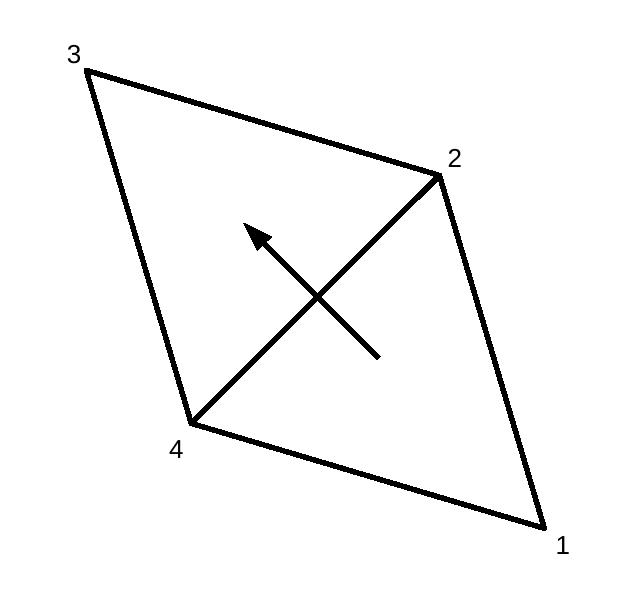
\includegraphics[scale=0.25]{figs/triangle.jpg}
 \caption{Node based edge flux method.} \label{scheme}
 \end{center}
 \end{figure}

At free stream boundaries, node values are set to the prescribed free stream values. At the wall boundary, the flux computation is done similarly as with interior edges, except flow tangency is enforced. Additionally, to maintain consitency in the control volume, the flux on a wall boundary edge is applied to the wall nodes as well. For interior nodes, the boundaries of the control volume surround the node (see figure \ref{fullcv}) so the scheme described above will ensure proper conservation at each node. However, at wall edges, a node resides on the control volume boundary (see figure \ref{wallcv}). As a result, the computed wall flux must be applied to the wall node as well to maintain conservation.

 \begin{figure}[htbp]
 \begin{center}
 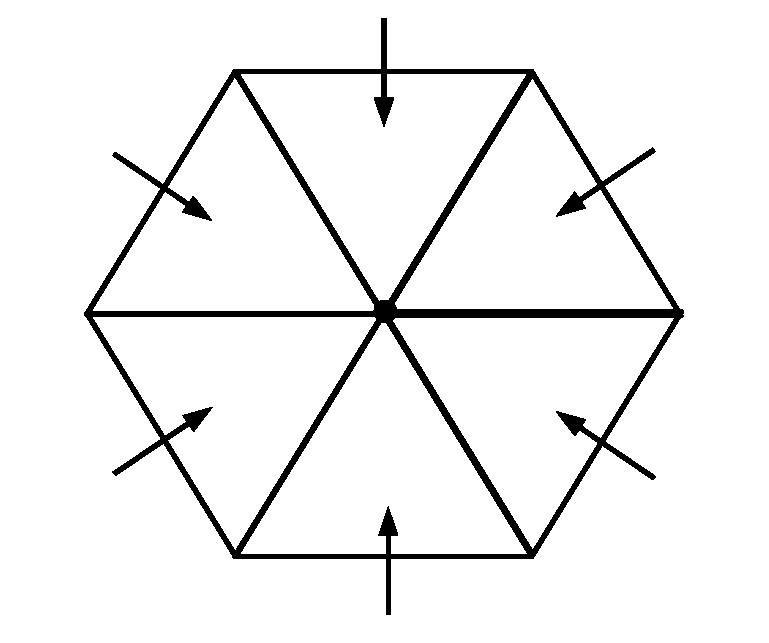
\includegraphics[scale=0.25]{figs/fullcv.jpg}
 \caption{Control volume around an interior node.} \label{fullcv}
 \end{center}
 \end{figure}

 \begin{figure}[htbp]
 \begin{center}
 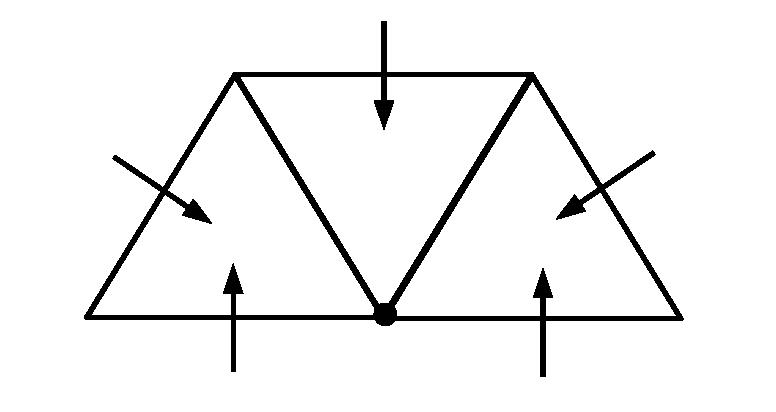
\includegraphics[scale=0.25]{figs/wallcv.jpg}
 \caption{Control volume around a boundary node.} \label{wallcv}
 \end{center}
 \end{figure}
 
In order to maintain stability in flows with shocks, a scalar artificial diffusion was added. The scalar diffusion was taken as the maximum eigenvalue of the Roe matrix and is applied everywhere in the flow. Although this method works, it is quite diffuse and leads to smeared shocks. There are two major issues with this method in terms of accuracy. First, the highest value of the Roe diffusion is used everywhere since the maximum eigenvalue of the Roe matrix is taken as the scalar. This leads to unncesssary diffusion in the majority of the domain. In addition, the artificial field is applied everywhere, whereas a more sophisticated method would detect and apply diffusion only to necessary areas (namely at shocks). 

 \pagebreak
 \section{Results}
 
 \subsection{Circular Arc}
 
 Transonic flow ($M_{\infty} = 0.9$) over a 5\% thick (at 50\% chord) circular arc bump was computed. Results showing contours of Mach number and pressure are below. In both plots, a supersonic region is visible over the bump (although the shock is visibly diffuse due to the use of first order scalar artificial diffusion). The surface pressure distribution shows that the shock is captured in approximately 5 points. Since the method is low order (especially the shock capturing scheme), a fairly fine triangulation was used.  


\begin{figure}[ht]
\centering
\subfigure[]{
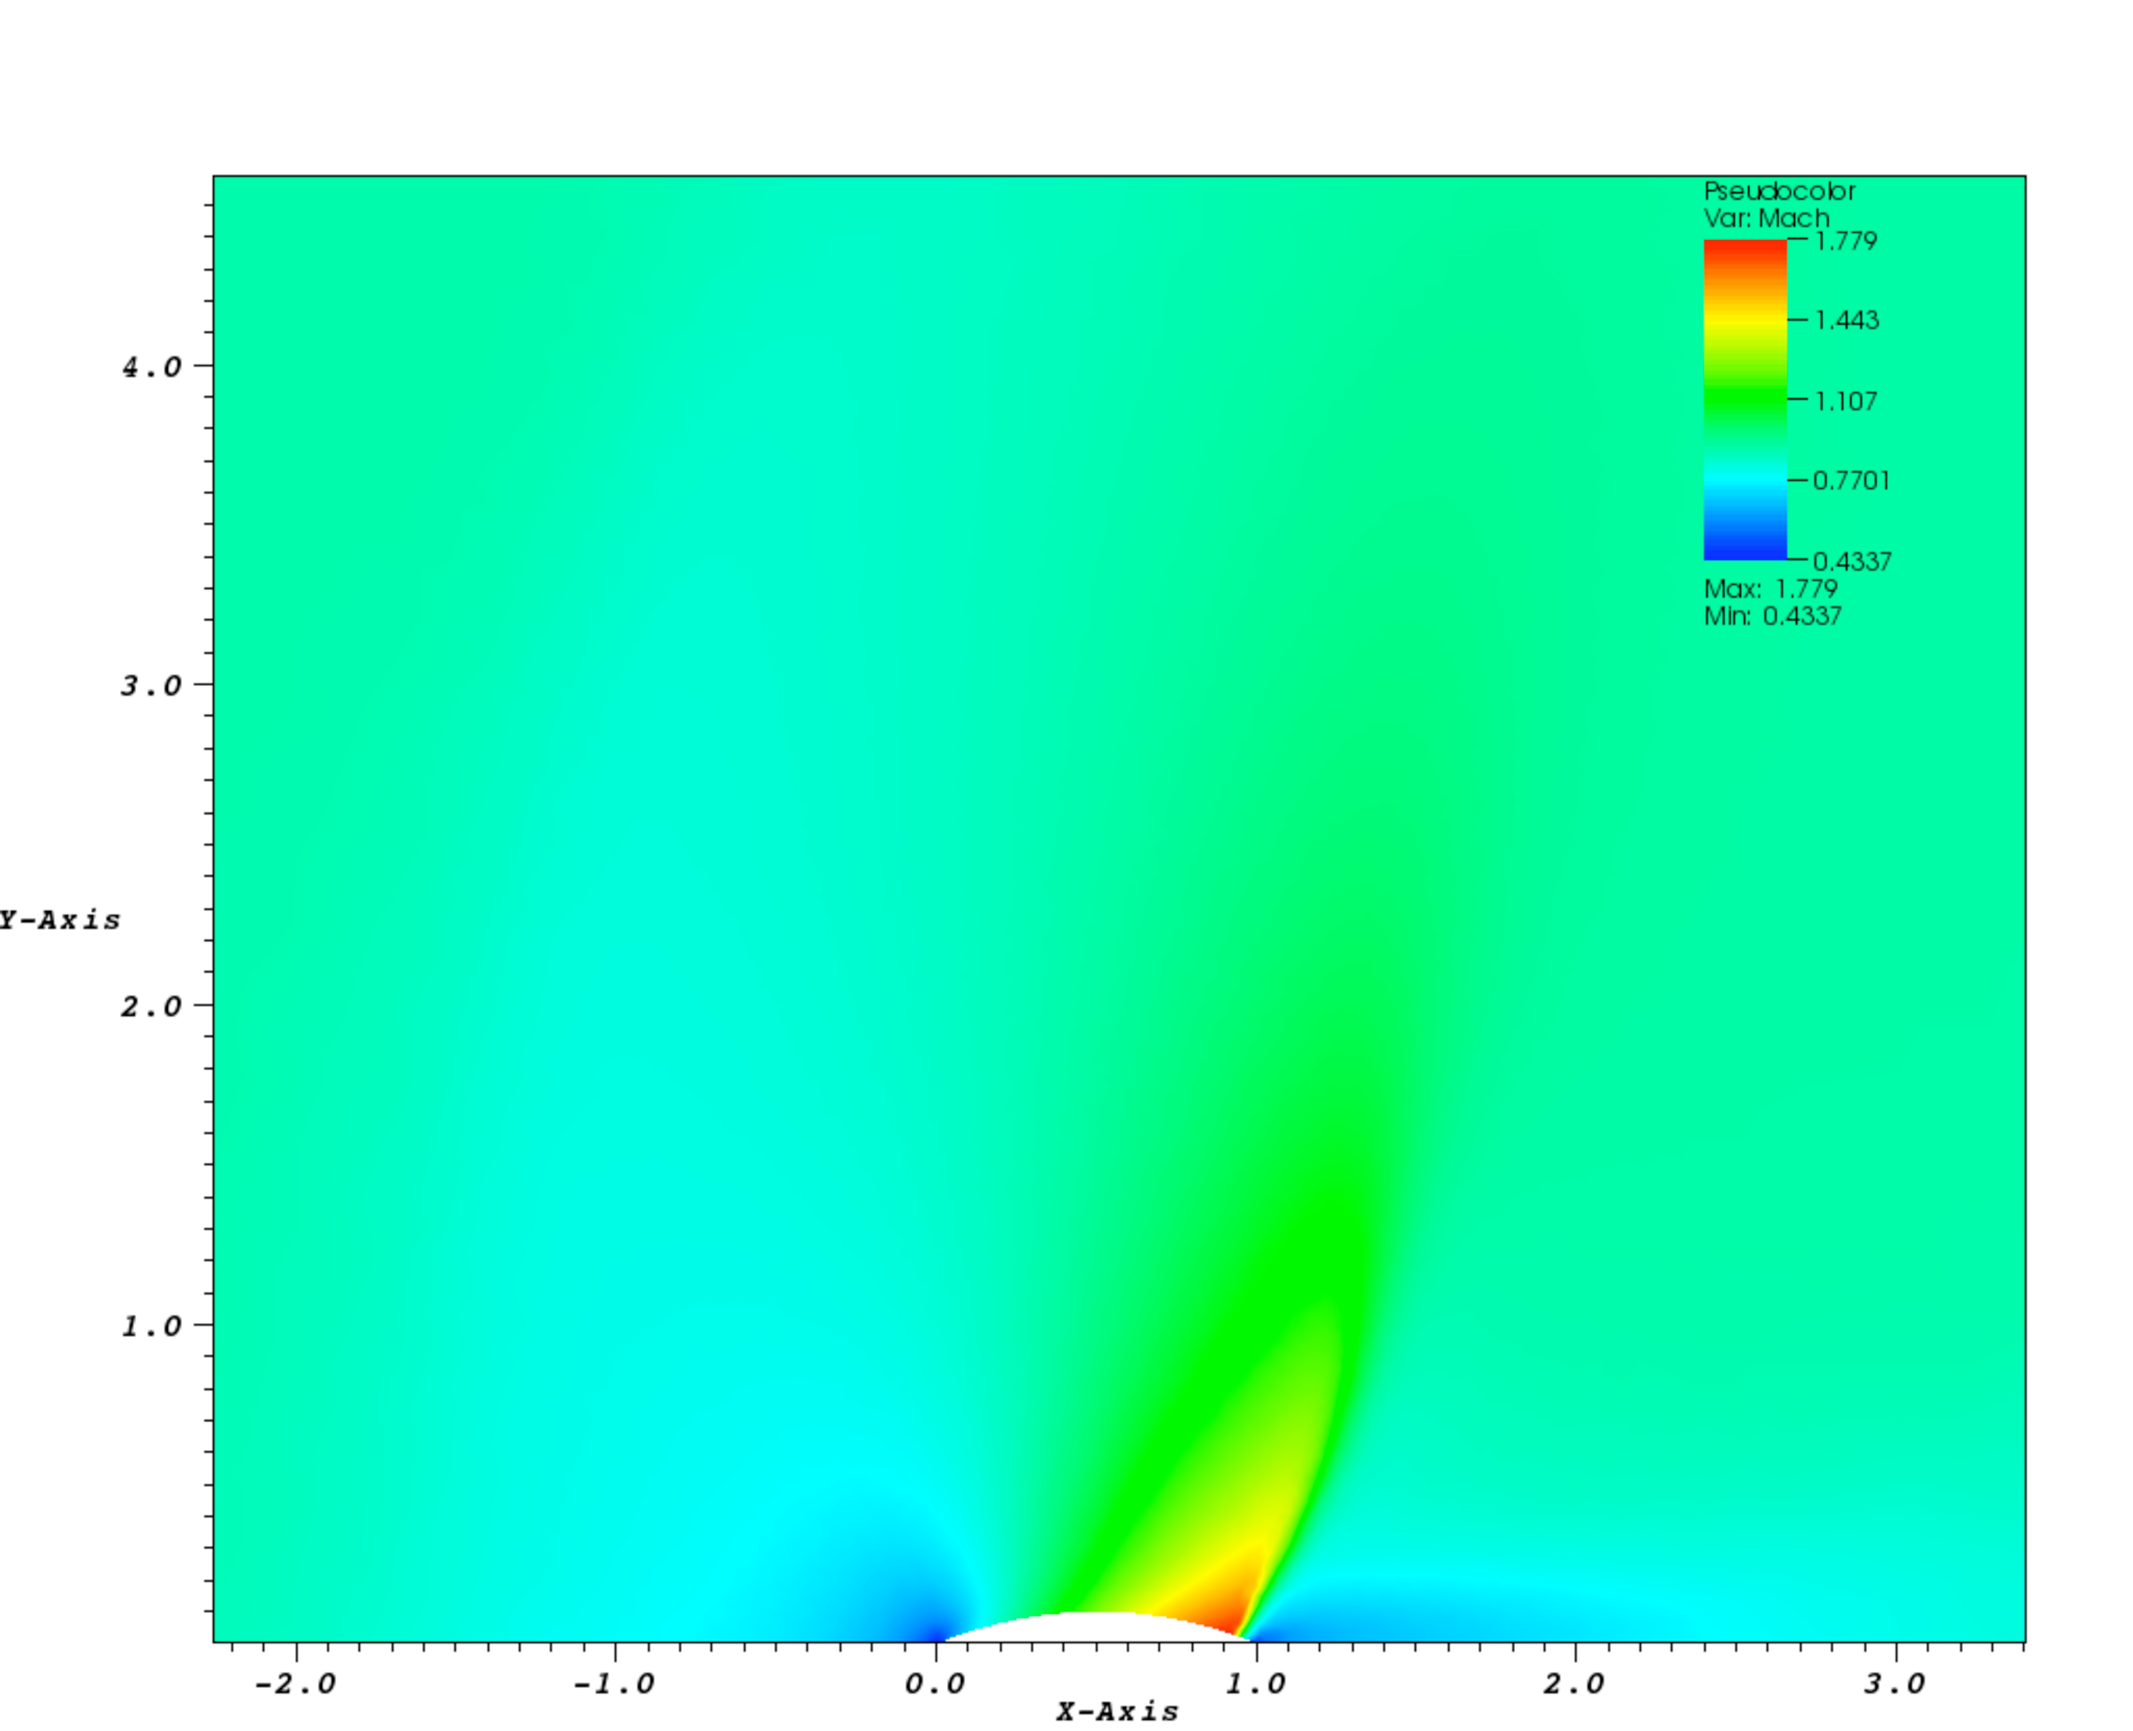
\includegraphics[scale=.2]{figs/bump_m_pc.pdf}
}
\hspace{-0.25in}
\subfigure[]{
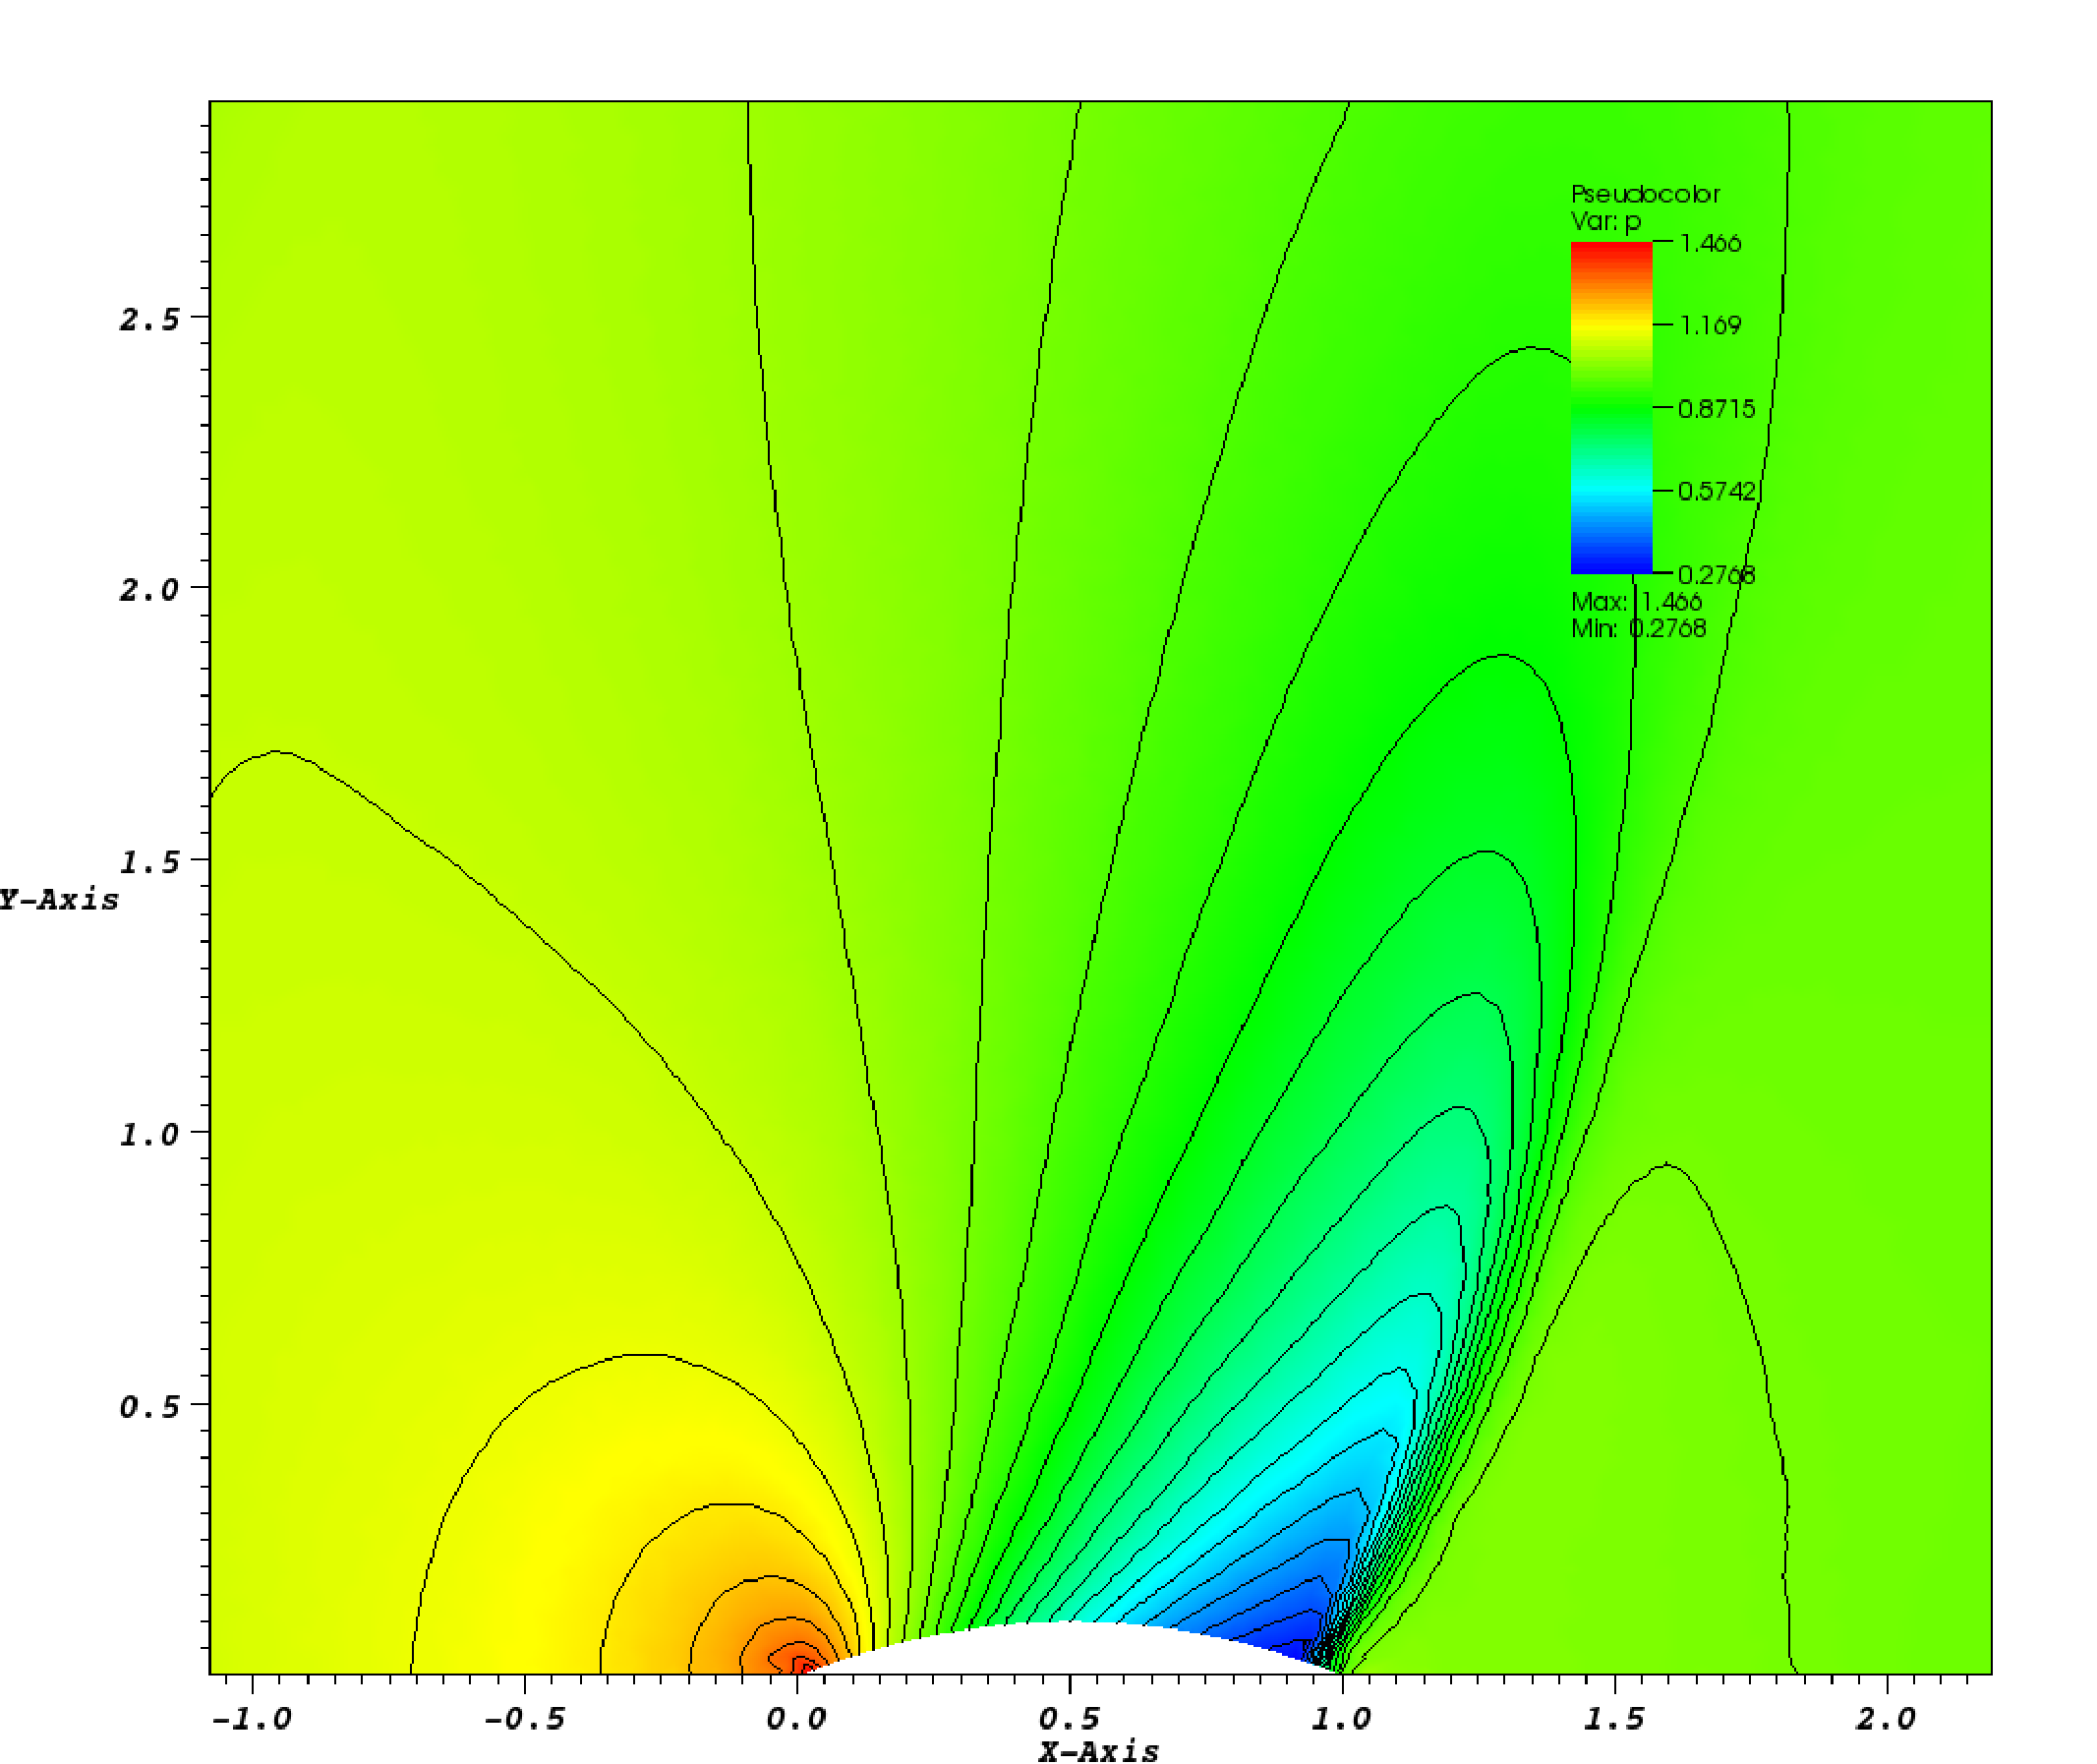
\includegraphics[scale=.2]{figs/bump_p_c.pdf}
}
\subfigure[]{
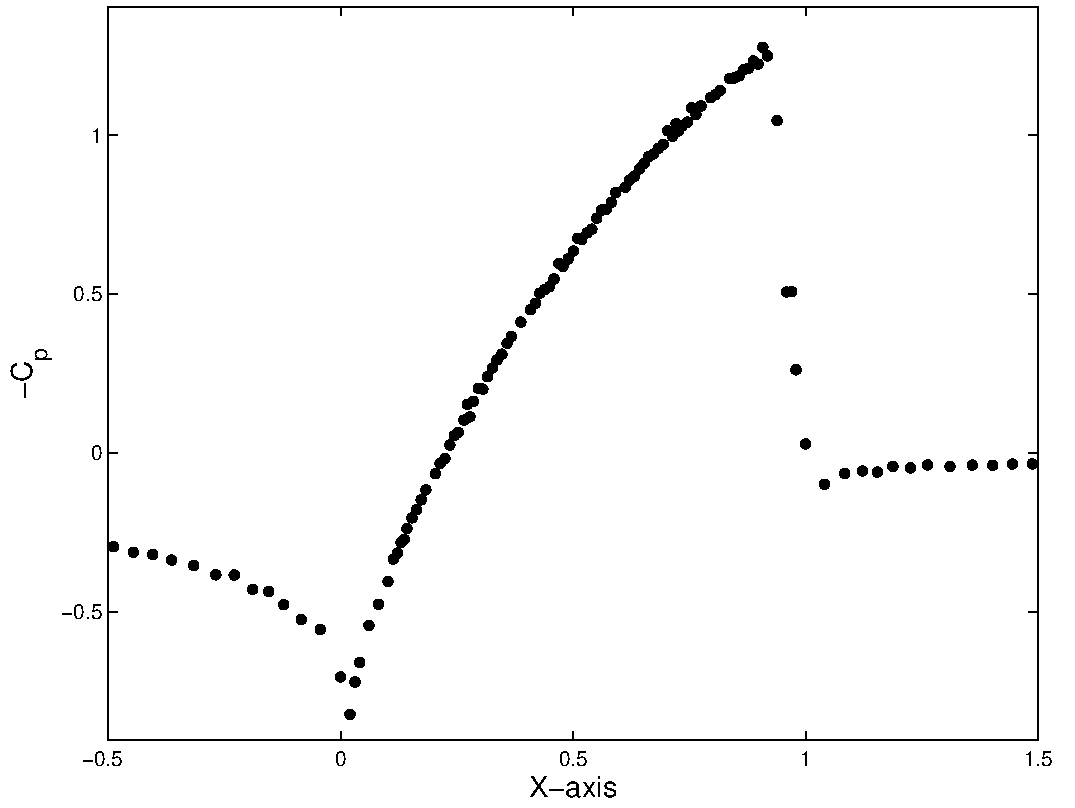
\includegraphics[scale=.4]{figs/bump_cp.pdf}
}
\hspace{-0.25in}
\subfigure[]{
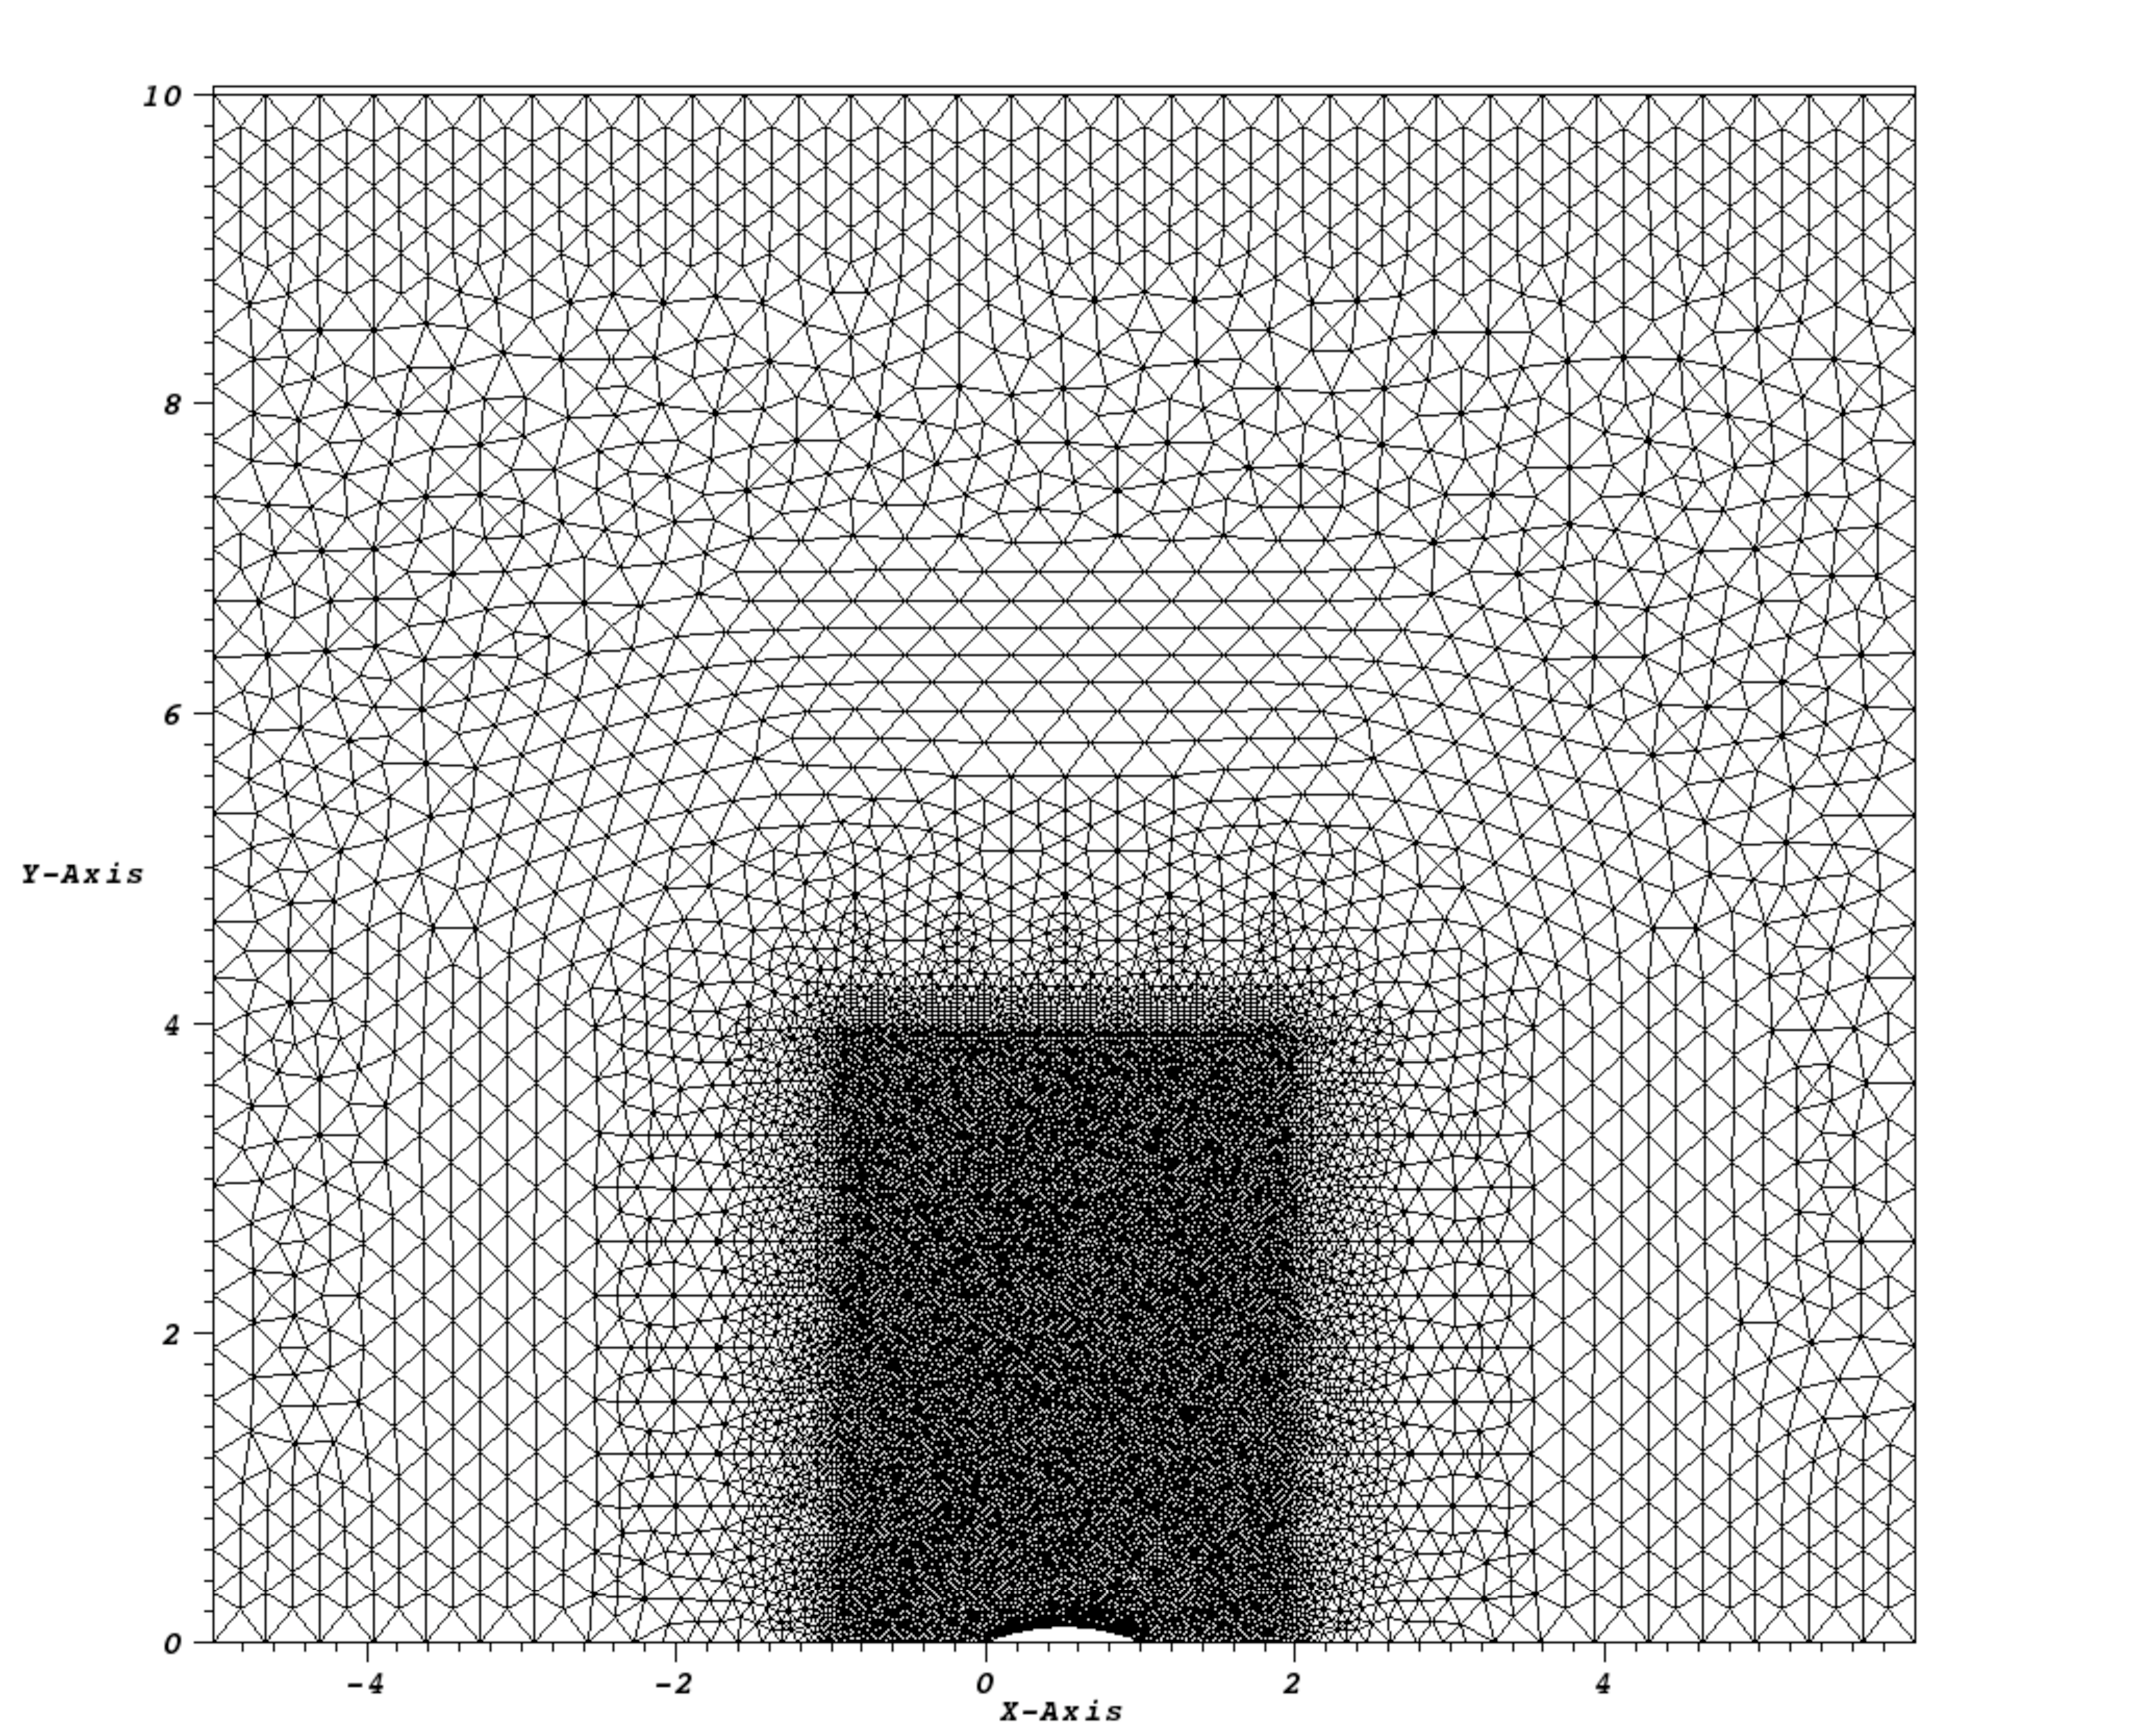
\includegraphics[scale=.2]{figs/bump_grid.pdf}
}
\caption{5\% Cicular arc foil. $M_{\infty}=0.9$}
\label{bump}
\end{figure}


 \pagebreak
 \subsection{NACA 0012}

Transonic flow ($M_{\infty} = 0.75$) over a NACA 0012 airfoil at $\alpha = 10^{\circ}$ was also computed. Contours of Mach number and pressure show a supersonic region on the upper surface of the airfoil. Again, due to the lower order of the method a relatively fine mesh was used to allow for a reasonable shock.

\begin{figure}[ht]
\centering
\subfigure[]{
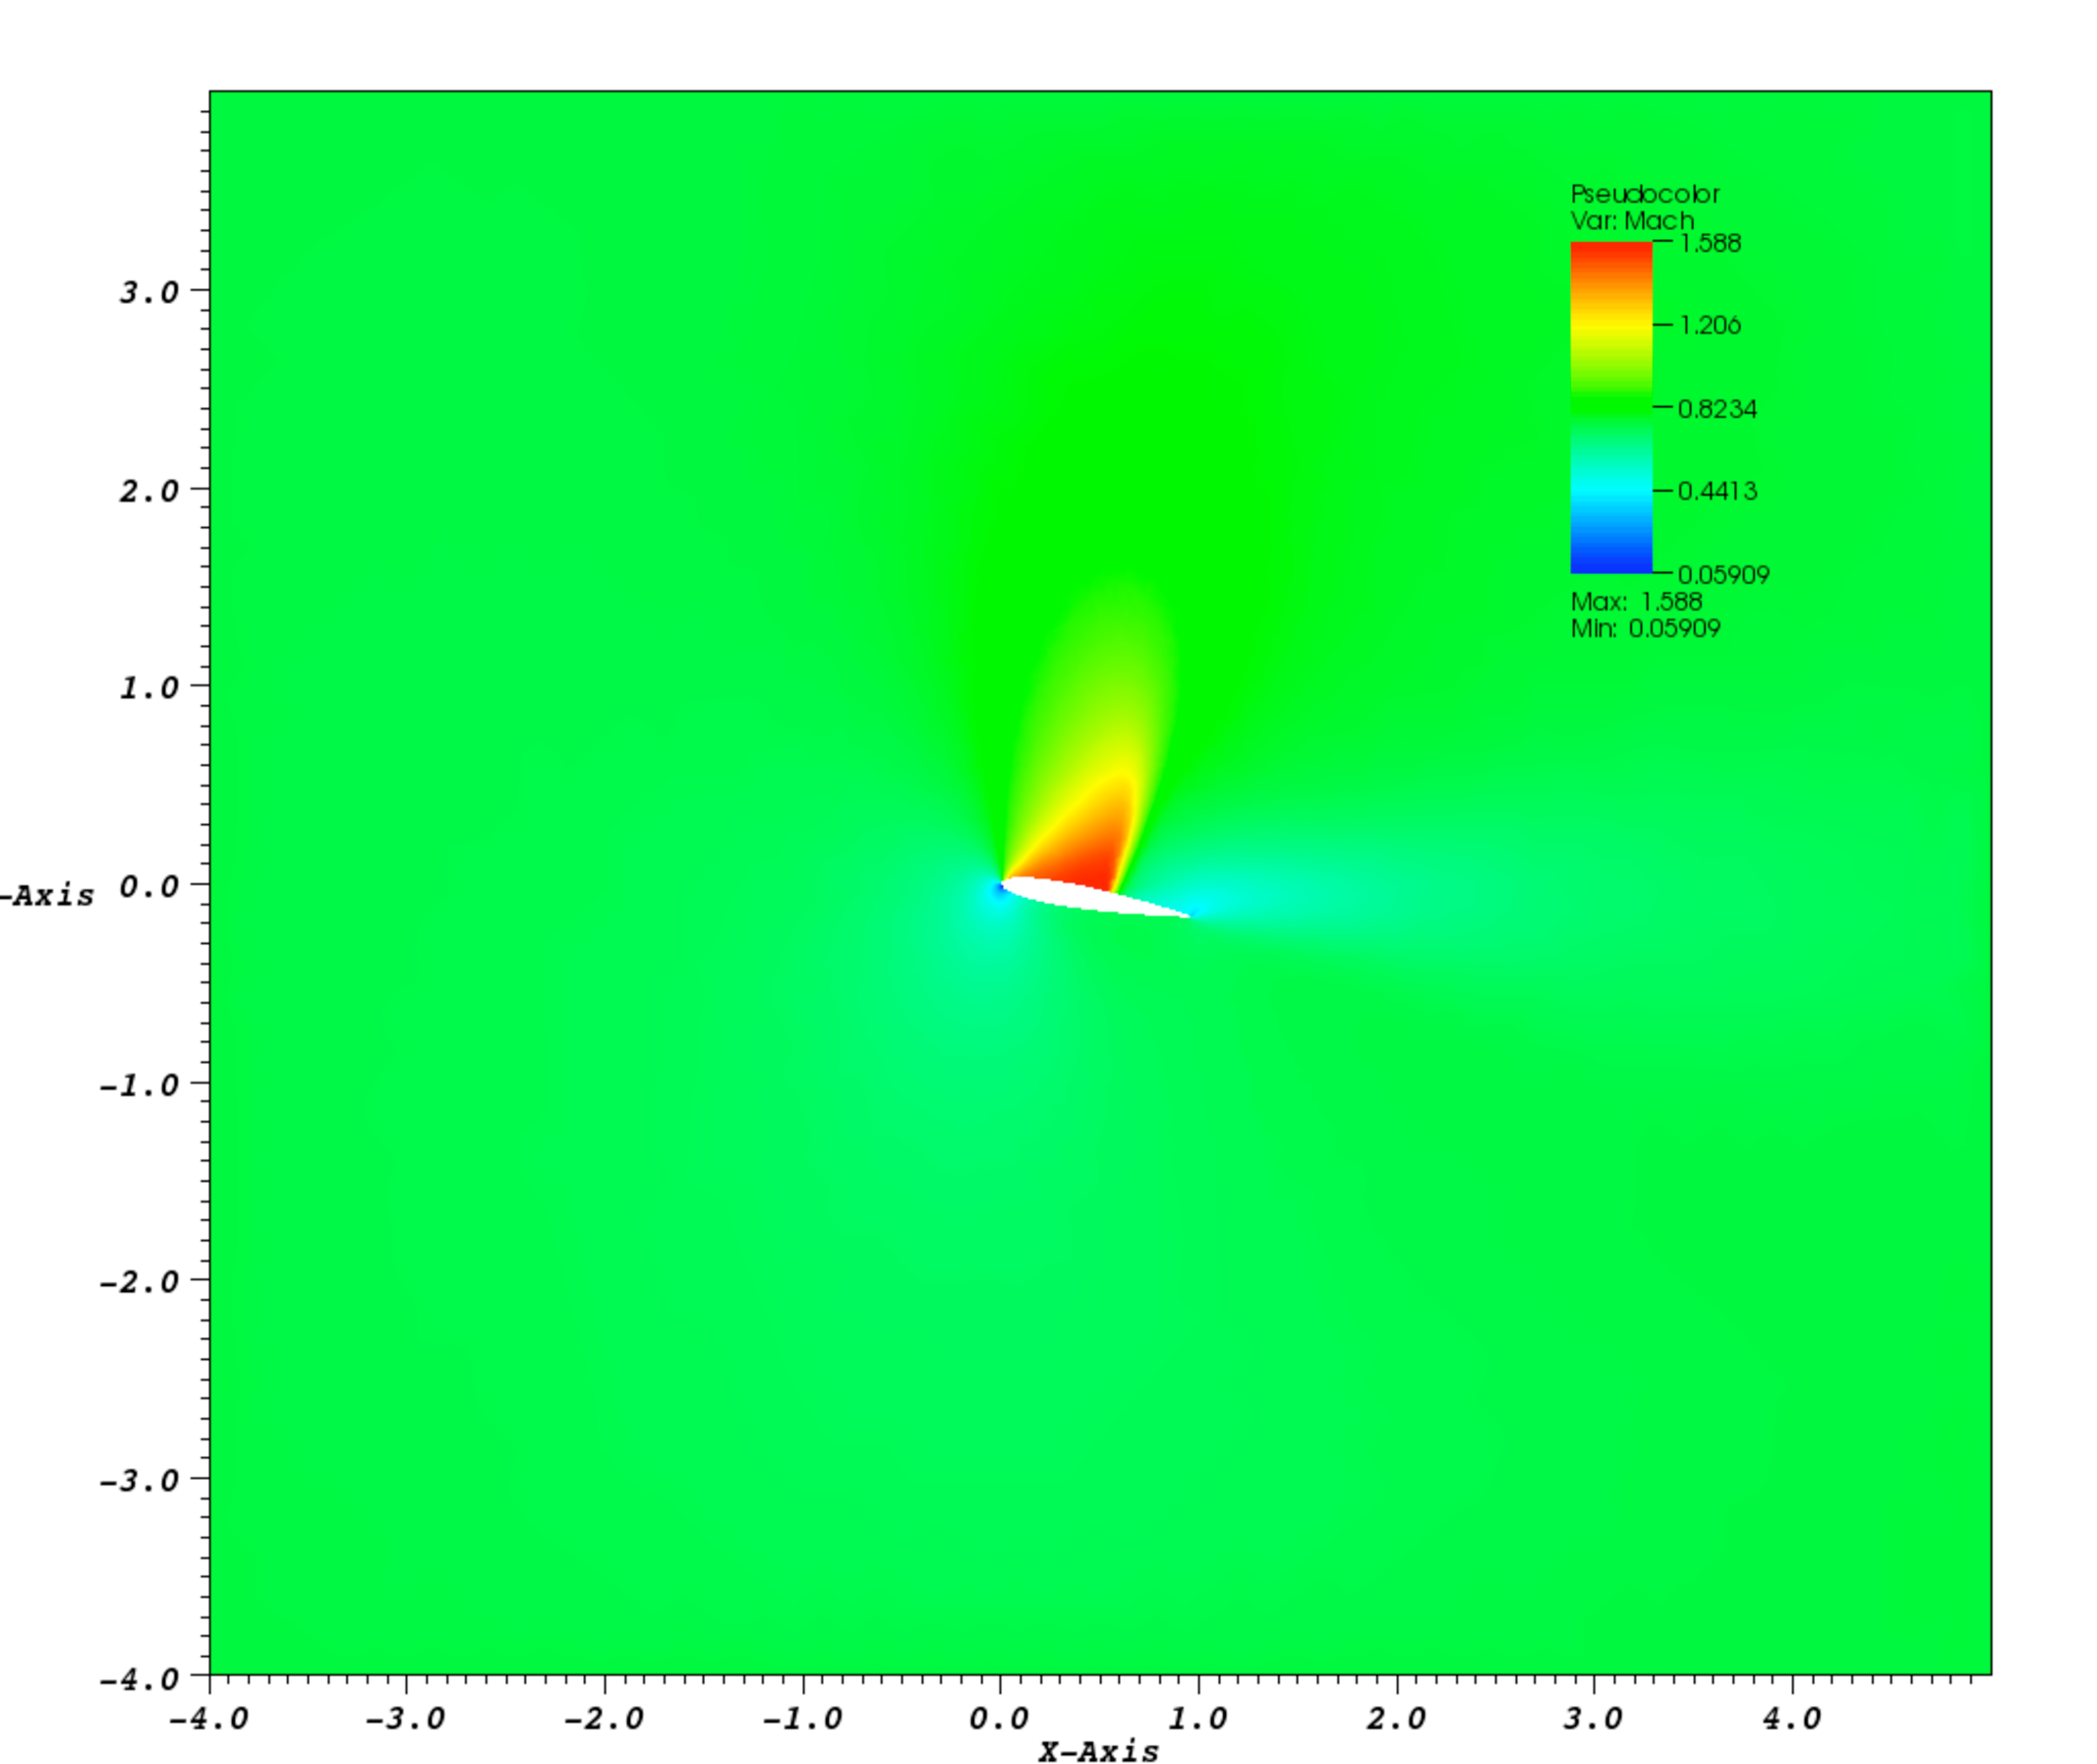
\includegraphics[scale=.2]{figs/naca_m_pc.pdf}
}
\hspace{-0.25in}
\subfigure[]{
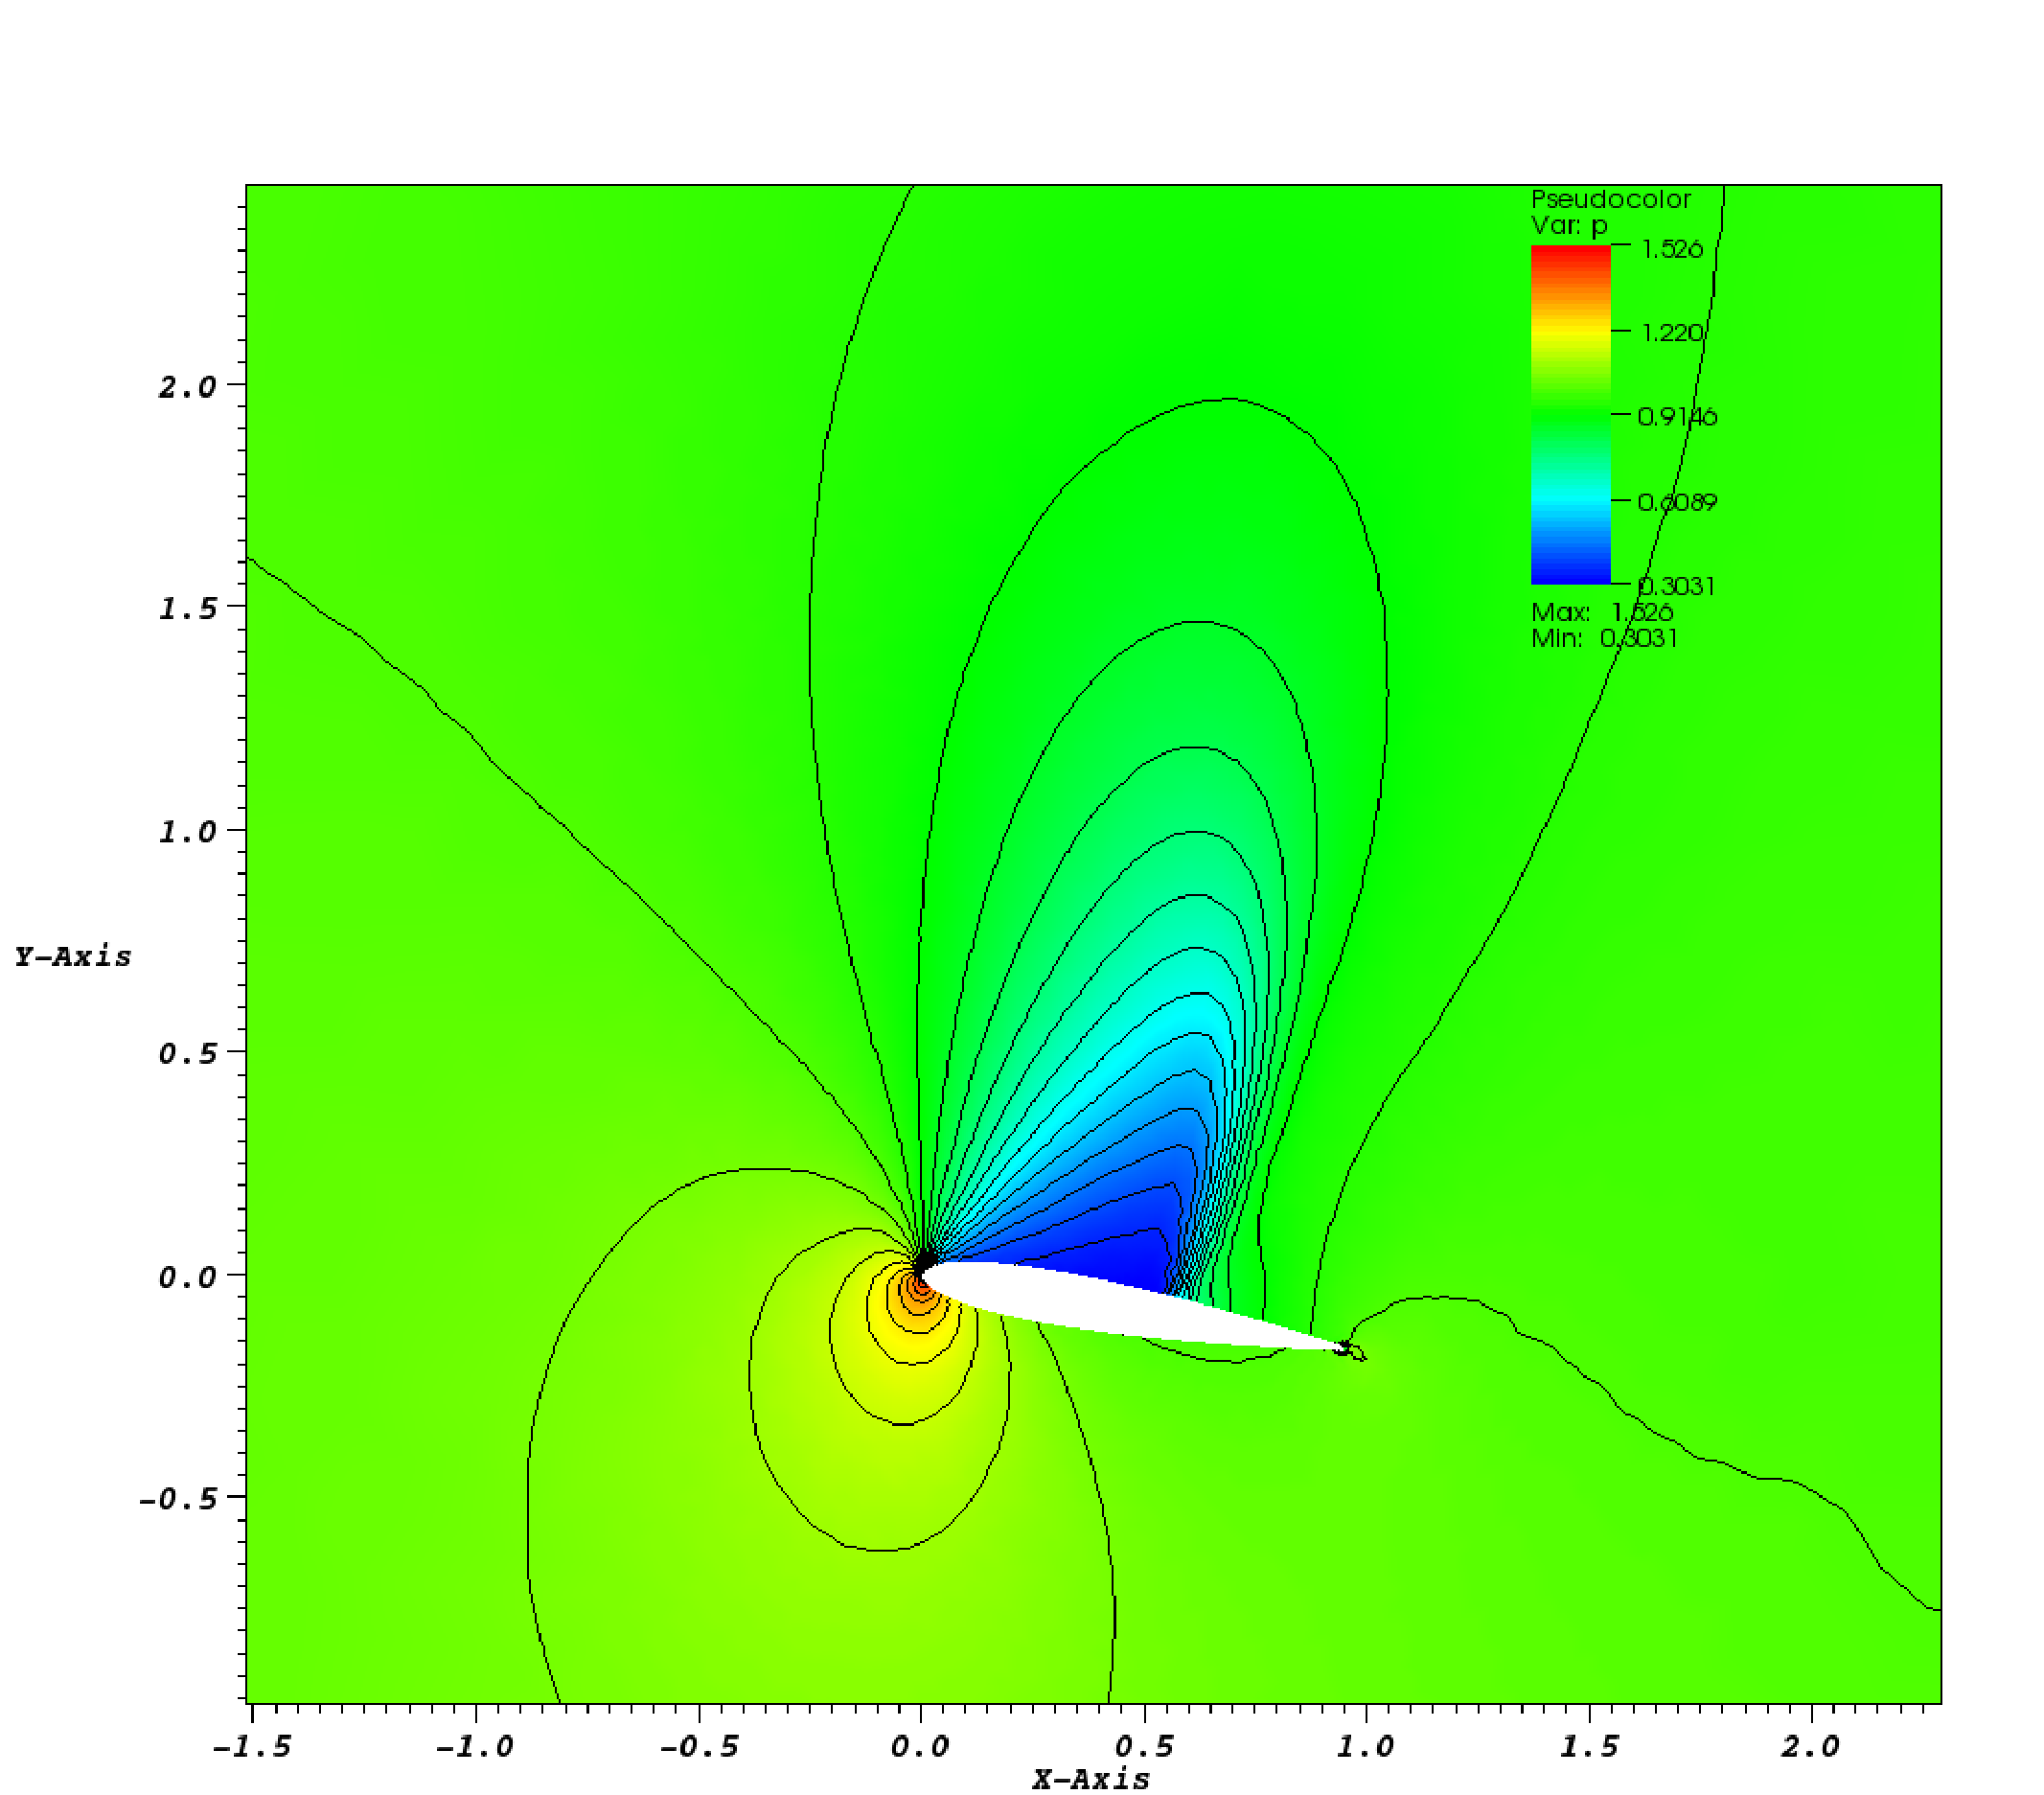
\includegraphics[scale=.2]{figs/naca_p_c.pdf}
}
\subfigure[]{
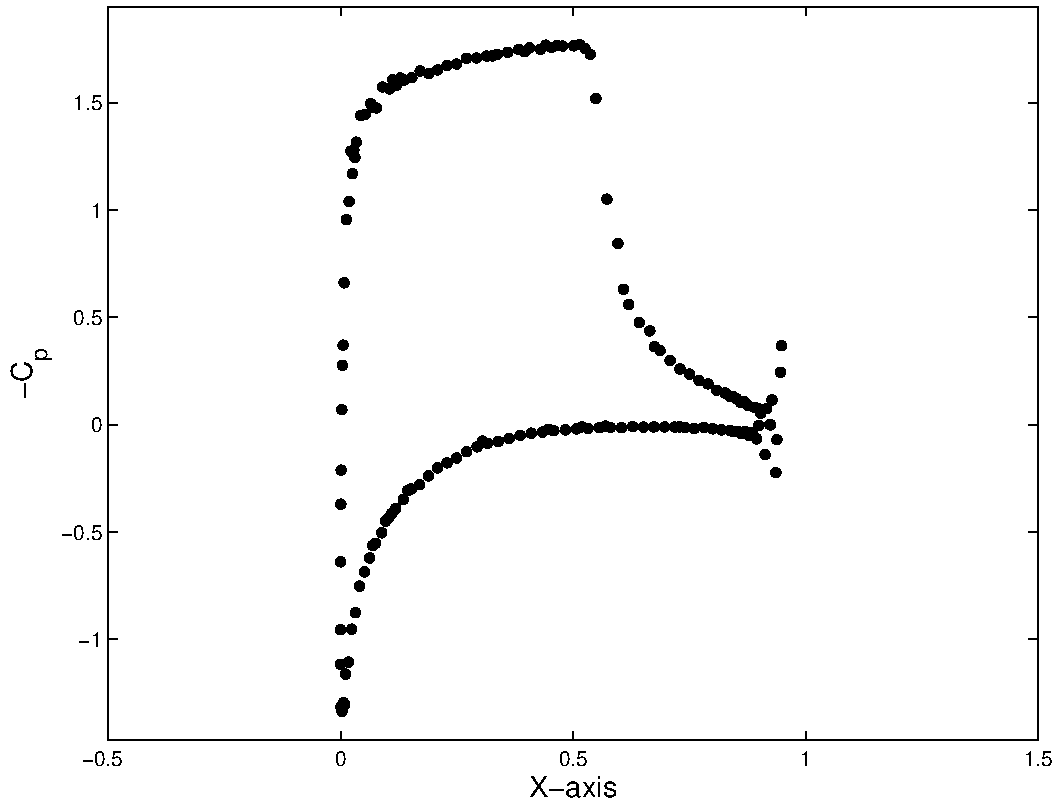
\includegraphics[scale=.4]{figs/naca_cp.pdf}
}
\hspace{-0.25in}
\subfigure[]{
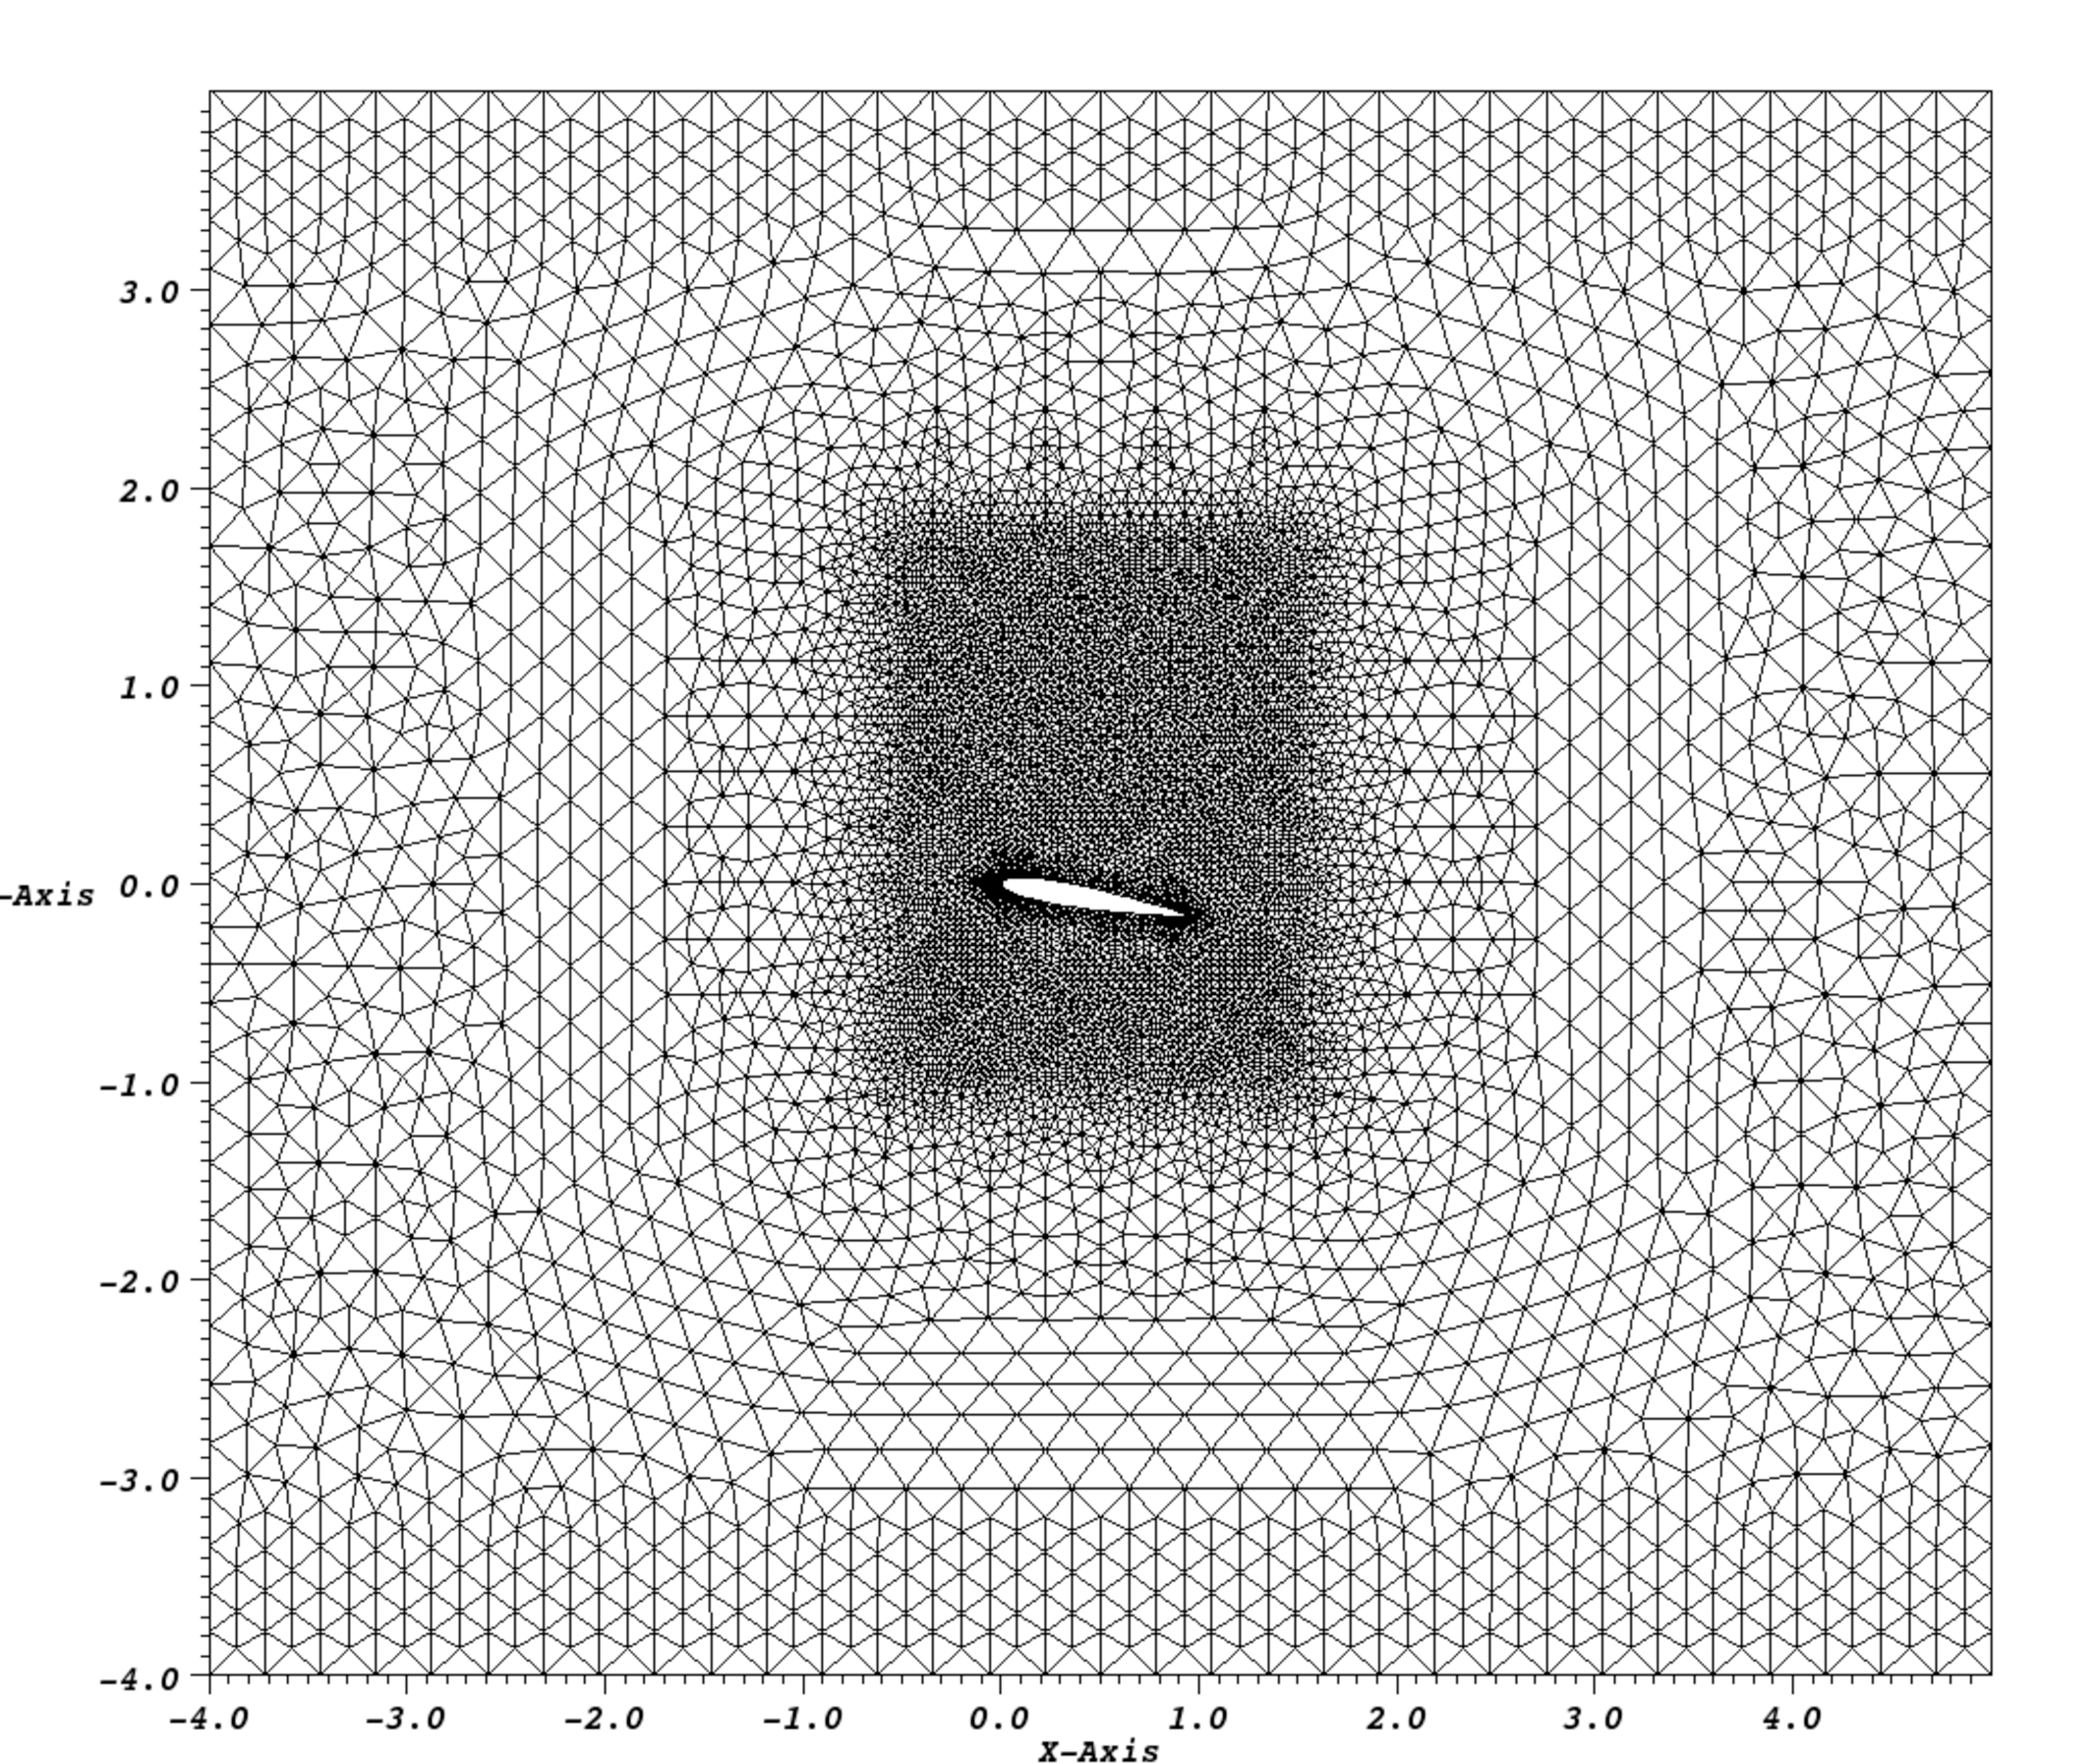
\includegraphics[scale=.2]{figs/naca_grid.pdf}
}
\caption{NACA 0012. $M_{\infty}=0.75$, $\alpha=10^{\circ}$.}
\label{naca}
\end{figure}

 \end{document}